\documentclass[11pt]{article}
\usepackage{fullpage}
\usepackage{mathpazo}
\usepackage[noend]{algpseudocode}
\usepackage{amsmath}
\usepackage{latexsym}
\usepackage{graphicx}
\usepackage{wrapfig}
\usepackage{bibentry}
\usepackage{bm}
\usepackage{qtree}
\usepackage{array}
\usepackage{eurosym}
\usepackage{textcomp}
\usepackage{tocloft}
\usepackage{makeidx}
\usepackage{rotating}
\usepackage{multirow}
\usepackage{multicol}
\usepackage{microtype}
\usepackage[font=footnotesize,labelsep=quad,labelfont=it]{caption}
\newcommand\subcaptionsize\footnotesize  % make this the same as the font size in the caption package
\newcommand\ignore[1]{}

\renewcommand\textfraction{0.0}
\renewcommand\topfraction{1.0}
\renewcommand\bottomfraction{1.0}

\newcommand\tightbox[1]{{\setlength\fboxsep{0pt}\framebox{#1}}}

\sloppy
\raggedbottom

\begin{document}


\section*{The Horde \\{\large Technical Report}}

\subsection*{Vittorio Ziparo and Sean Luke}

%\begin{figure}
\begin{wrapfigure}{r}[0in]{3in}
\vspace{-2em}
\begin{center}
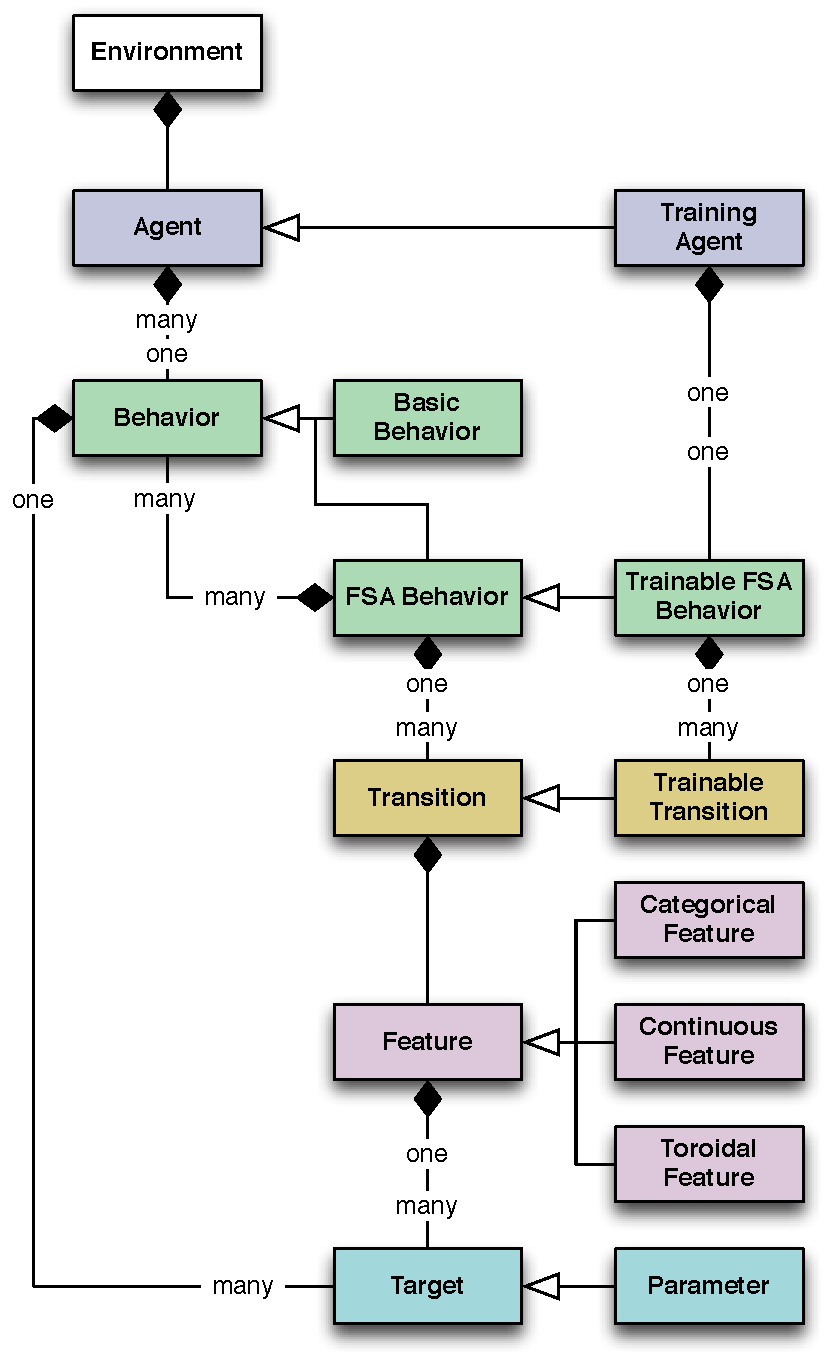
\includegraphics[width=3in]{UML.pdf}
\end{center}
\vspace{-2em}
\caption{UML diagram of the basic Horde objects and relationships.}
\vspace{-2em}
\label{uml}
%\end{figure}
\end{wrapfigure}

The Horde system consists of one or more {\bf agents} wandering about in an {\bf environment} consisting of other agents, obstacles, food, markers, etc.  Each agent employs one {\bf behavior}: and multiple agents may share the same behavior.  At most one of those agents is the {\bf training agent}.  This is an agent whose behavior is being trained by the user.  At the beginning of the simulation the agent calls the {\it start} method of the behavior to let it know it's being used.  Each timestep the agent pulses his behavior once, which causes the agent to perform that behavior for that timestep.  Finally, at the end of the simulation the agent calls the {\it stop} method of the behavior.

\subsubsection*{Behaviors and Transitions}

Behaviors take various forms.  First, there are {\bf basic behaviors}.  These are atomic, hard-coded behaviors provided by the system.  For example, the behavior {\it rotate left} might be a basic behavior: when employing this behavior, the agent will spin to the left some number of degrees per timestep.

Second, there are {\bf FSA behaviors}.  These may also be hard-coded behaviors but are not atomic.  Instead they consist of Moore-machine style finite-state automata.  Each node in the FSA is a behavior: and transitions from node to node are triggered based on features of the environment.  The behavior performed by an FSA is the current state that it is in.  For example, were our agent employing the wall-following FSA behavior shown in Figure \ref{fsa}, and that FSA was presently in the {\it rotate-left} state, the agent would be performing the {\it rotate-left} behavior.  One state defined as the {\it initial state} in which the FSA begins.  Any state could be the initial state; though we chose to define a special do-nothing behavior called {\it start} which is always the initial state, and which always transitions immediately to some other state.

Node transitions take the form of rules which are or are not true about the environment.  We presume that all transitions leaving a node constitute a set of disjoint rules.  If no such rule is true, no transition is triggered and the FSA stays in its present state.  For example, were our FSA presently in the {\it forward} behavior (moving forward), and an obstacle was in front or less than 2.3 units to the left, we would transition to the {\it rotate right} behavior and start rotating to the right.  On the other hand, if no obstacle was in front and an obstacle was further than 5.2 units to the left, we would transition to the {\it rotate left} behavior.  Finally, if neither of these were true, we would continue moving forward.  All transitions leaving a given state are collectively embodied in a single {\bf transition} object associated with that state: thus an FSA behavior with \(N\) states also has \(N\) transition objects.  

\begin{wrapfigure}{r}[0in]{3in}
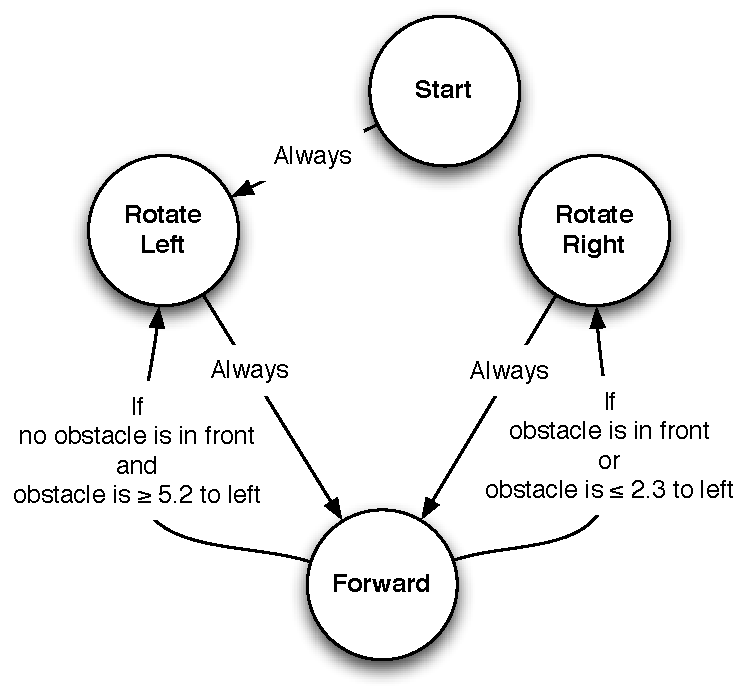
\includegraphics[width=3in]{WallFollower.pdf}
\caption{A simple FSA for wall following (counter-clockwise).}
\label{fsa}
\end{wrapfigure}


Behaviors inside the FSA receive the same start, stop, and pulse messages as any behavior would.  When an FSA's {\it start} behavior is called, it transitions to its initial state and calls {\it start} on the state's underlying behavior.  Likewise when an FSA's {\it stop} behavior is called, it calls {\it stop} on its current state's underlying behavior.  When an FSA behavior is pulsed, it does three things.  First, it pulses, once, the behavior corresponding to its current state.  Second, it calls the state's corresponding transition object and receives from it a new state to transition to; this of course could be the current state itself.  Third, if the FSA is transitioning to a new state, it calls {\it stop} on the old state, then {\it start} on the new state.

Importantly, {\bf FSA behaviors can be nested:} that is, there's no reason that one or more of the behaviors corresponding to states in the FSA are themselves FSA behaviors.  This allows the creation of hierarchical FSAs, and ultimately, behavior libraries.  No recursion is permitted however.  Because of this hierarchical nesting, each time a top-level FSA is pulsed, ultimately this pulse is propagated down to a single basic behavior, which is the behavior the agent actually performs.

One special behavior that we have found useful in FSAs is what we call the {\it done} behavior.  This behavior signals a ``done'' flag in its {\it grandparent} FSA and, then immediately transitions to the {\it start} state (no other transition is permitted).  The purpose of the done behavior is to signal to the grandparent that the parent FSA has completed its task: it is ``done'', which is why it transitioned to the done behavior in the first place.  This flag, which is reset when the grandparent transitions away from the parent FSA behavior, is presented to the grandparent as a feature which it can use in making transition decisions.

\subsubsection*{Features and Targets}

A transition object for a state consists of a set of rules which indicate which new state the FSA should transition to.  These rules rely on feature of the world.  For example, the test ``an obstacle is further than 5.2 to the left'' relies on a {\bf feature}, perhaps called {\it distance to closest obstacle on the left}.  Features may be queried for their current values (in this case, perhaps ``2.1'').  In our system features presently take three forms: {\bf categorical features}, which return values like ``red'' or ``blue''; {\bf continuous features}, which return real-valued numbers (like distances); and {\bf toroidal features}, which return real-valued numbers but which are assumed to wrap around in a toroidal fashion (like angles).  Boolean features are typically modeled as categorical features.  One boolean feature is the {\it done} feature, which returns whether or not the done flag has been triggered.

Importantly, Horde supports behaviors and transitions which are general-purpose.  Rather than create a behavior which goes ``to obstacle number 42'', we can create a behavior which goes ``to X'', where X may be specified later.  This is done first by separating the notion of features and behaviors from the {\bf targets} to which they apply.  For example, a feature (like distance or angle) may be either specified with regard to {\it ground targets} (``obstacle 42'' or ``the closest obstacle on my left'')\,---\,resulting in a feature such as ``distance to obstacle 42''\,---\,or it the target may simply be left unspecified (``distance to X'') , to be bound to a ground target at some later time.  In the latter case, the target is called a {\bf parameter}.

Basic behaviors may also be similarly parameterized.  Additionally, when an FSA behavior is created, all parameters of features and behaviors within the FSA must be either bound to ground targets or bound to the FSA's own parameters.  In the latter case the FSA behavior itself becomes a parameterized behavior.

\subsubsection*{Training}

The above mechanism is sufficient to hand-code hierarchical FSA behaviors to do a variety of tasks; but Horde was meant instead to enable the {\bf learning} of such tasks.

This is done by assigning one agent in the environment to be the {\bf training agent}, as associating that agent with a special FSA behavior called a {\bf trainable FSA behavior}.    The trainable FSA behavior is more or less like an FSA behavior except that all available behaviors form states in the FSA, and the transitions have been replaced with {\bf trainable transition} objects.

Even though all available systems form states, this doesn't mean that they'll be used: initially all the trainable transitions are ``empty'', meaning they solely transition to their own states.  Thus the entire FSA graph is disconnected.  Only as the user adds training information to the FSA does it start creating transitions from state to state; but only to those states which the user actually requested.  Ultimately the remaining states are discarded or ignored.

Each trainable transition employs a machine-learning classification algorithm to determine which state to transition to.  Though in theory there is no reason we couldn't have used a K-nearest-neighbor, Support Vector Machine, or other classification algorithm, in our experiments we have settled on employing a variant of C4.5 Decision Trees to do this task.  Decision trees have many disadvantages, but certain advantages of use to us: first, many subspaces in the feature space of our agent approximately take the form of rectangular regions.  Second, our features employ unscaled toroidal, continuous, and categorical data, which is straightforward for decision trees but somewhat nontrivial for other algorithms.

The training process works like this.  The agent starts in the ``start'' state (doing nothing), and the user is provided with a collection of buttons or keystrokes, each associated with a certain available behavior.  The user then directs the agent to do various things in the environment by pressing the buttons/keys, similar to controlling an agent in a game. When the agent is presently performing a behavior \(S\) and the user chooses a new behavior \(S'\), the agent transitions to this new behavior and records a data element, known as an {\it example}, of the form \(\langle S, \vec{F}, S'\rangle\), where \(\vec{F}\) is a vector of all current feature values at the time of transition.

Immediately after the agent has transitioned to \(S'\), it turns out to be often helpful to record an additional example of the form \(\langle S', \vec{F}, S'\rangle\).  This adds at least one ``default'' (that is, ``stay in state \(S'\)'') example, and is nearly always correct since in that current world situation the user, who had just transitioned to \(S'\) would nearly always want to stay in \(S'\) rather than instantaneously transition away again.

At the end of a training session, the user then turns off training, which causes Horde to build decision trees from the example data.  For each behavior state \(S\), Horde builds a decision tree \(D_S\) based on all examples of the form \(\langle S, \vec{F}, S'\rangle\).  The decision tree treats a vector \(\vec{F}\) as the input values and the new state \(S'\) as the output class.  If there are no examples at all (because the user never transitioned from \(S\), often because he likely never transitioned {\it to} it in the first place), the decision tree is simply defined as always transitioning back to \(S\).

Thus determining which new state to go to is essentially a classification task based on the current world situation.  At the end of this process, Horde has built some \(N\) decision trees, one per state.  The agent can then be left to wander about in the world on its own, using the FSA defined by the behaviors and these decision trees.

Because the potential number of features can be very high, and many unrelated to the task, and because we want to learn based on a very small number of samples, we wish to reduce the dimensionality of the input space to the machine learning algorithm.  This is done by allowing the user to specify beforehand which features will matter to train a given behavior.  For example, to learn a Figure-8 pattern around two unspecified targets A and B, the user might indicate a desire to use four parameterized features: {\it distance to A}, {\it distance to B}, {\it direction to A}, and {\it direction to B}.  The resulting learned behavior will have two parameters (A and B), which must ultimately be bound to use it in any meaningful way later on.

If A and B are unspecified, how were they defined during training?  After all, to gather relevant example data about the distance to A, {\it something} had to be A.   This is done by temporarily binding them to existing objects in the world (typically obstacles, other agents, or simple location markers).  The user can specify what these temporary bindings are.

We note that equating behaviors with states is not sufficient for a general Moore-machine FSA: in a real Moore machine, multiple states may perform the same behavior.  Thus if there is only one ``go to A'' button, two states which require going to A will require special handling.  Horde deals with this in one of two ways.  First, Horde might permit multiple buttons which do the same behavior (but which represent separate states in the FSA).  Second, it's straightforward to train a simple one-state FSA which simply does ``go to A''.  This FSA can then be named, say, ``go to A number 2'' and be included along with ``go to A'' for the user to use: they're different states (technically different behaviors) but ultimately do exactly the same thing.

\paragraph{Toroidal Features} We pause to note how we implemented toroidal features in decision trees.  Because angular regions are so common (and are toroidal), toroidal features are important.  The decision tree performs splits on toroidal regions much like it performs splits on continuous regions: by sorting the data by feature value and then finding the lowest-information split.  However whereas continuous splits involve finding a single split point \(A\) and breaking the examples into values \(< A\) versus \(\geq A\), toroidal splits instead involve finding {\it two} split points \(A\) and \(B\), with \(A < B\), and breaking the data into values \(v\) for which \(A \leq v < B\) and values which are either \(< A\) or \(\geq B\).  We term these groups ones which are ``inside'' and ``outside'' the split respectively.  We realize the cost of finding not one but two split values increases the computational complexity of finding an optimal split point by an additional \(O(n)\).  Though we doubt our approach here is original (and have not looked very hard), we have so far not found any other use of toroidal splits in the decision tree literature.

\begin{figure}
\begin{center}
\noindent\begin{tabular}{cc}
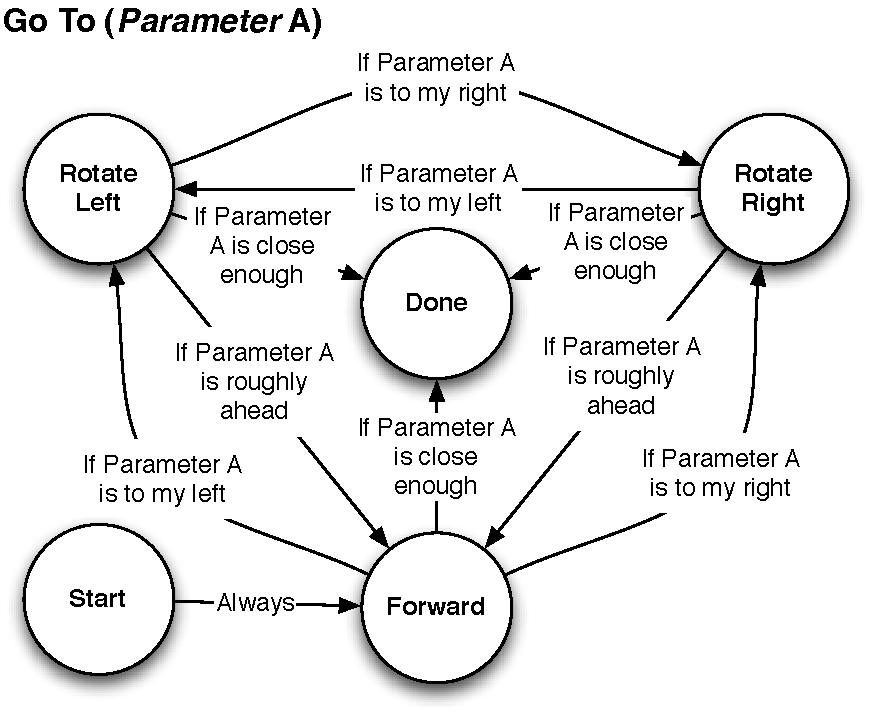
\includegraphics[width=3.5in]{GoTo.pdf}&
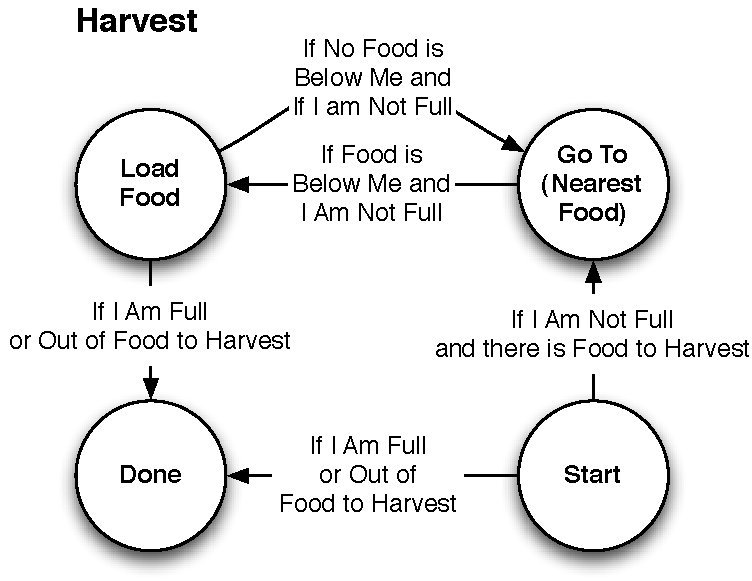
\includegraphics[width=3in]{Harvest.pdf}\\
\\
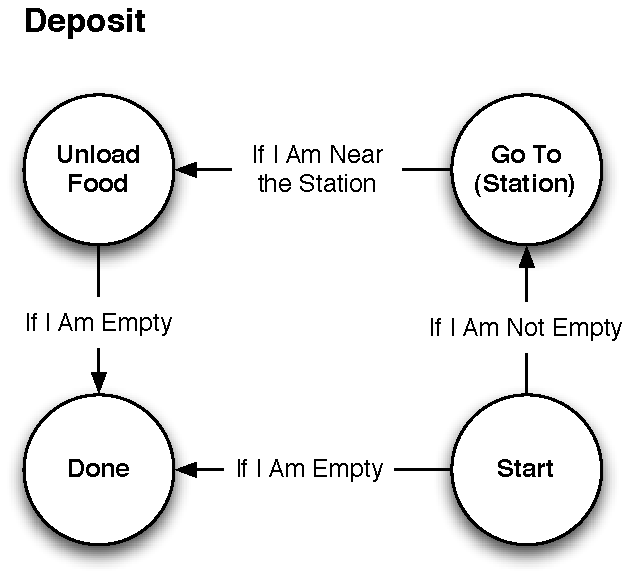
\includegraphics[width=2.6in]{Deposit.pdf}&
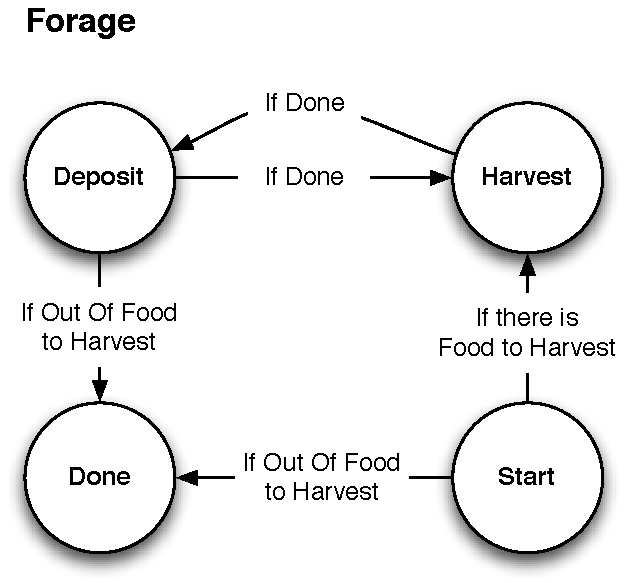
\includegraphics[width=2.6in]{Forage.pdf}\\
\end{tabular}
\end{center}
\caption{The Forage behavior and its sub-behaviors: Deposit, Harvest, and GoTo({\it Parameter} A).}
\label{foraging}
\end{figure}

\subsubsection*{Putting it Together: an Example}  We have successfully trained the agent to perform a moderately complex foraging task: to harvest food from food sources and bring it back to deposit at the agent's central station.  Food can be located anywhere, as can the station. Food at a given location can be in any concentration, and depletes, eventually to zero, as it is harvested.  The agent can only store so much food before it must return to the station to unload its harvest.  If the agent depletes food at a harvest location before it is full, it continue harvesting at another location before returning.

Foraging tasks are of course old hat in robotics, and foraging behaviors are not particularly difficult to code by hand.  But {\it training} such a behavior is more challenging.  We selected this task as an example because it illustrates a number of features special to Horde: our foraging behavior is in fact a three-layer FSA hierarchy; employs ``done'' states; involves real-valued, toroidal, and categorical (boolean) inputs; and requires one behavior with an unbound parameter used in two different ways.

The behavior is shown in Figure \ref{foraging}.  It requires six basic behaviors: {\it Start} and {\it Done}, go {\it Forward}, {\it Rotate Left}, {\it Rotate Right}, {\it Load Food} (deplete the current location's food by 1, and add 1 to the agent's stored food), and {\it Unload Food} (remove all the agent's stored food).  It also requires several sensor capabilities: {\it distance to A}, {\it angle to A}, {\it amount of food below me} (that is, located here), {\it amount of food stored within me}, and {\it food remains in the environment}.  Finally, we require two targets: the {\it station} and {\it nearest food}.

From this we build a hierarchy of four FSA behaviors:

\begin{itemize}
\item {\bf The Go To ({\it\textbf{Parameter}} A) Behavior}\quad This behavior causes the agent to go to the object marked A.  The behavior is a straightforward bang-bang servoing controller: rotate left if A is to your left, else rotate right if A is to your right; else go forward.  When close enough the agent enters ``done'' behavior state, which raises the Done flag and reverts to the ``start'' state.  It's not really necessary to include the ``done'' flag as the higher level behaviors don't use it; but we did so for good measure.  The Go To behavior is employed, as a behavior state, by both of the next two behaviors.

We trained the Go To behavior by temporarily declaring a marker in the environment to be Parameter A, and reducing the features to two: distance (continuous) and angle (toroidal) to Parameter A.  We then placed the agent in various situations with respect to Parameter A and ``drove'' it over to A by pressing keys corresponding to the rotate left, rotate right, and forward behaviors.  When the agent was roughly on top of A, we pressed the ``done'' key.  Each time we pressed a key, Horde records examples as described earlier, then performs the desired transition. 

\item {\bf The Harvest Behavior}\quad This behavior causes the agent to go to the nearest food, then load it into the agent.  When the agent has filled up, it signals that it is done.  If the agent has not filled up yet but the food has been depleted, the agent goes to a new food location and continues.  This behavior used the previously-learned Go To behavior as a subsidiary state behavior, binding its Parameter A to the {\it nearest food} target.  This behavior employed the features {\it amount of food below me} (continuous), {\it amount of food stored within me} (continuous) and {\it food remains in the environment} (categorical).  

We trained the Harvest Behavior by pressing buttons to instruct the agent to go to the nearest food, then load it, then (if appropriate) signal ``done'', else go get more food.  We also placed the agent in corner-case situations (such as if the agent started out already filled up with food).

\item {\bf The Deposit Behavior}\quad This behavior causes the agent to go to the station, then unload its food and signal that it is done.  If the agent was already empty when starting, it would immediately signal done.   This behavior also used the previously-learned Go To behavior as a subsidiary state behavior, but instead bound its Parameter A to the {\it station} target.

We trained the Deposit Behavior in a similar manner as the Harvest Behavior: by pressing buttons to go to the station and unload food, and constructed situations to handle corner cases appropriately.

\item {\bf The Forage Behavior}\quad This behavior causes the cycle between depositing and harvesting, unless there is no more food in the environment,  Accordingly, this behavior employed the previously-learned Deposit and Harvest behaviors.

We trained the Forage Behavior in a similar manner as the Harvest and Deposit Behaviors: by pressing buttons to instruct the agent to deposit and harvest food as appropriate.  The behavior used the {\it food remains in the environment}, {\it amount of food below me}, and {\it amount of food stored within me} features.

\end{itemize}


\subsubsection*{Current Issues}

The proof of concept works nicely: we can train parameterized, hierarchical behaviors for a variety of tasks.  But there are a number of interesting issues, big and small, that remain to be dealt with.

\paragraph{Where to place the split value in the decision tree}  When a decision tree splits on a continuous attribute, it must decide on what the critical decision value is.  Commonly this value is half-way between the neighboring values among the examples.  For example, if the examples had attribute values of 0.1, 0.3, 0.9, and 1.0, and the split was between the 0.3 and 0.9, then the decision value might be defined to be 0.6.  For our environment this is often a bad choice.  For example, suppose an agent is going to a target, and when the agent reaches the target it changes its behavior.  We might have a few examples early on as it's going to the target, then one or two right at the target.  If the attribute was distance-to-target, our values thus might look like: 102 100 60 53 [split] 3 2 2 1.  The current value strategy would define the critical value to be 28 (that is, (53+3)/2).  This is a terrible value: it instructs the agent to change its behavior when it's 28 units away from the target, when we really want it to change when it's right at the target (about 3 or less).

The obvious way to deal with this is to move the critical value over to the 3.  But it may not be immediately obvious to the learner whether to move it to the 3 or to the 53 just based on the order of the example as they arrive.   Different scenarios might want the split point in different places (near the 53, or near 28).  Assuming we always want it near 3, we could place it at 90\% of the way to 3, and perhaps decide on 3 because it happened after the 53.

Another approach is to continuously insert ``continue doing what you're doing'' examples automatically as the agent goes about its task.  Thus when the user indicates a change, the difference between that change and the most recent ``continue'' example will be small, and even if the critical value were based on the average between the two, that average would be close to the new ``change'' example.  The system has this capability at present, and the user can also add ``continue'' examples by repeatedly pressing keystrokes as well.

\paragraph{Pruning}  We are entirely unsatisfied with decision tree pruning results.  We've tried various traditional post-hoc pruning methods and also pre-pruning approaches.  Nothing seems to work very well: they're highly sensitive in our problem --- change the pruning weight slightly and the whole tree collapses to something very small (and very poor).

\paragraph{Unlearning} There are two major reasons why an agent may make a mistake.  First, it may have learned poorly due to an insufficient number of examples or unfortunately placed examples.  Second, it may have been misled due to {\it bad examples}.  This second situation arises due to errors in the training process, something that's very easy to do!  When an agent makes a mistake, the user can then jump in and correct it by immediately pressing buttons or keystrokes.  This causes the system to drop back into training mode and add those examples to the behavior's collection.  However it does {\it not} cause any errant examples to be removed.  It's an interesting research problem to identify exactly which examples are improper and whether, or how, to remove them.

\paragraph{The Done Behavior}  It's not yet clear how to handle the Done behavior.  Should the Done behavior immediately transition to the Start behavior?  (that's what we're doing now).  Or should it simply transition to a null behavior where the agent stops operating?  Or should the agent continue doing what it was doing prior to entering the Done behavior?  Should there be multiple Done behaviors, indicating different end states (success vs. failure, for example)?

It's also not entirely clear when or if the Done state is useful.  A raised Done flag might be helpful in training agents to transition to somewhere else when a behavior is ``done'', but checking for a completed condition is often just as easy to do at the higher level --- run a behavior until something happens of interest (the agent reaches a given destination) and transition at that point, rather than transitioning when the behavior thinks it's done.

\subsubsection*{Future Tasks}

\paragraph{Multiple Agents}  Our immediate next goal is to move to training multiple agents.  In the general case, multiagent learning is a much more complex task than single-agent learning, involving game-theoretic issues which may be well outside the scope of this project.  However we believe there's lots of interesting areas: for example teaching agents to perform actions as {\bf homogeneous behavior} groups (perhaps by training an agent with respect to other agent not under his control).  Another area of multiple agent training may involve {\bf hierarchies of agents,} with certain agents in control of teams of other agents.

\paragraph{Programming versus Training}  Our goal has been to train agents rather than explicitly code them.  However we also aim to do so with a minimum of training.  These goals are somewhat in conflict.  If we throw the agent in the world and expect him to learn, several factors can cause the agent to take a very long time to learn.  First, if the size and dimensionality of the feature space is large, the agent may require more samples to nail down in which regions certain transitions are warranted.  Second, if the complexity of the FSA is high, the agent may also require large numbers of samples to learn it.

To deal with this we have ways of countering these problems.  First, the system explicitly permits task decomposition, which is essentially a method for breaking a complex FSA into multiple much simpler FSAs.  Second, the system allows the user to explicitly specify the feature space for a given FSA, thus limiting it to those features the user thinks are relevant.  Note that both of these cases begin to smell like {\it programming}: the user is figuring out to some degree the procedure for the agent to follow (via decomposition) and what features are relevant to the agent to figure out the solution. 

So the question we face is: how much explicit specification can we provide before this ceases to really be a learning example?  We need to find the sweet spot between the efficiency of programming and the convenience (and elegance) of training and learning.

\paragraph{Other Representations}  FSAs cannot straightforwardly do parallelism or planning.  We chose FSAs largely because they were simple enough to make training intuitively feasible.  Now that we've demonstrated this, we may wish to consider how to train with more sophisticated representations, such as petri nets or hierarchical task network plans.

\paragraph{Making a Game}  From the outset we imagined that this whole project would make a good game in and of itself.  Hence the name {\bf \textit{The Horde}}: the idea was that you as the Guru would train stupid, simple agents to do tasks, then more complex tasks, then work as a group waging war against other users' hordes.  Sounds fun, yes?

\end{document}